\section{SimpleKMeans}\label{SimpleKMeans}
Beim Clustern des AT auf dem Testrechner wurden in Abh�ngigkeit von Attributanzahl und Anzahl der Cluster folgende Ausf�hrungszeiten erzielt.

\begin{figure}[htp]
\centering
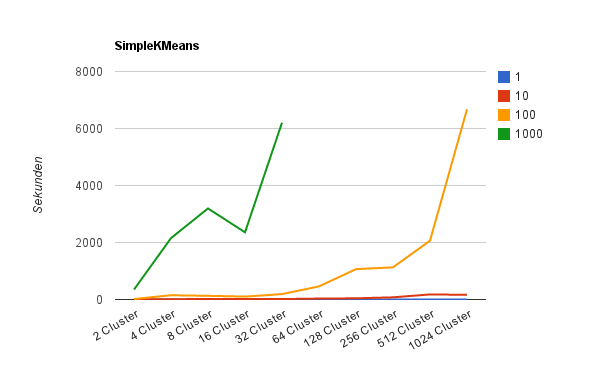
\includegraphics[width=1\textwidth]{Ingo/Bilder/SimpleKMeans.png}
\caption{Ausf�hrungszeiten von SimpleKMeans}
\label{fig:SimpleKMeans}
\end{figure}

In dem Diagramm ist erkennbar, dass die Ausf�hrungszeit steigt, je mehr Attribute und je mehr Cluster es gibt.
Auf einem einzelnen Rechner dauert das Clustern des AT f�r 1000 Attribute und 8 Clustern schon eine knappe Stunde.
F�r mehr Attribute oder mehr Cluster st��t der Testrechner an seine Grenzen.